\documentclass[specialist, 12pt, href]{article}
\usepackage[utf8]{inputenc}
\usepackage[russian]{babel}
\usepackage[T2A]{fontenc}
\usepackage{indentfirst}

\usepackage{latexsym,amssymb,amsthm}
\usepackage{amsfonts}
\usepackage{amsmath}
\usepackage{graphicx}
\usepackage{subfigure}

\usepackage[a4paper, includefoot,
            left=2cm, right=2cm,
            top=2cm, bottom=2cm,
            headsep=1cm, footskip=1cm]{geometry}

\usepackage{hyperref}
\setcounter{tocdepth}{2}
\allowdisplaybreaks[4]

\linespread{1.2}
\title{Принципы активного обучения}
\author{Иванова Елизавета}
\date{}

\begin{document}
\maketitle

\subsection{Введение}

Большинство задач машинного обучения, которые мы встречаем, относятся к
обучению с учителем или без учителя.
Предположим, что в нашей конкретной задаче обучения с учителем есть
некоторая функция, которая сопоставляет ответ любому объекту из
неразмеченных данных, но при этом является дорогостоящей процедурой
(достаточно дорогой, чтобы не обращаться к ней постоянно). Будем
называть ее \emph{оракулом}. Тогда основная идея \emph{активного обучения} ---
выбирать объекты среди неразмеченных данных так, чтобы минимизировать кол-во вызовов
оракула.

\begin{figure}[htbp]
\centering
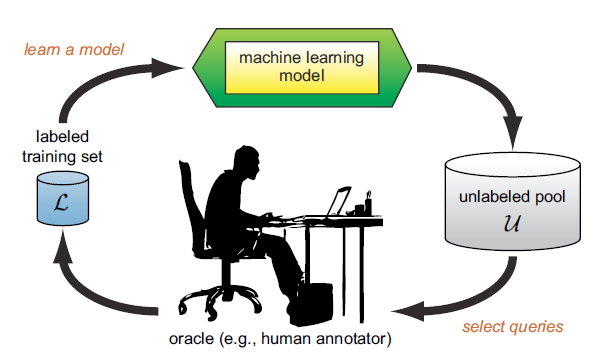
\includegraphics[width=5in]{img/al.png}
\caption{Схема активного обучения (семплирование из пула)}
\end{figure}

Активное обучение применяется в любой области, где построение обучающей
выборки затратная процедура. Если вы занимаетесь классификацией текстов,
изображений и т.п., найти неразмеченные данные не составляет труда. Но
готовые размеченные датасетами, которые подходят под вашу задачу, найти
сложнее, приходится размечать самому, или просить друзей, или обращаться
в специальные сервисы (Яндекс.Толока, Amazon Mechanical Turk). Друзей
сильно мучить не хочется, а сервисам нужно платить, поэтому здесь
пригодится активное обучение.

\paragraph{Почему это
работает?}

Прежде чем перейти к теоретическим аспектам, давайте рассмотрим два
примера, демонстрирующих, почему имеет смысл выбирать объекты для
разметки и построения обучающей выборки.

\emph{\textbf{Пример 1.}} Дана функция
\(g(x, \theta) = \mathbb{I}_{x > \theta}(x),\, x \in [0, 1],\, \theta \in [0, 1]\),
и нужно оценить \(\theta\), при условии, что мы можем вычислять
\(g(x, \theta)\) в произвольных точках \(x\), но процедура эта крайне
дорогая, и кол-во вызовов хочется сделать как можно меньше.

Наивный подход --- взять для разметки равномерную сетку
\(\{i/n\},\, i = 1,\ldots, n - 1\). Оценка по времени этого решения ---
\(O(n)\) измерений.

\begin{figure}[htbp]
\centering
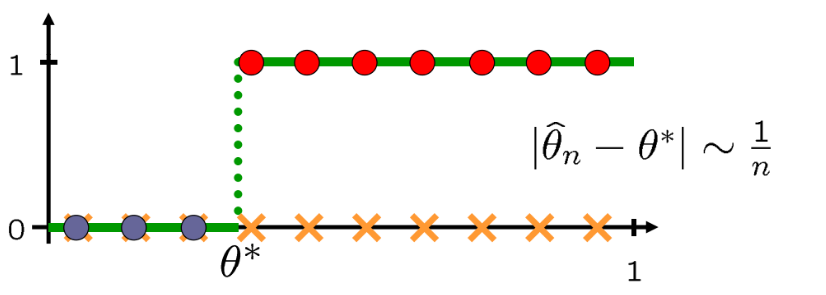
\includegraphics[width=4in]{img/naive.png}
\caption{Задача линейного разделения. Наивный подход}
\end{figure}

Но быстрее эта задача решается двоичными поиском, временная сложность
которого \(O(\log n)\).

\begin{figure}[htbp]
\centering
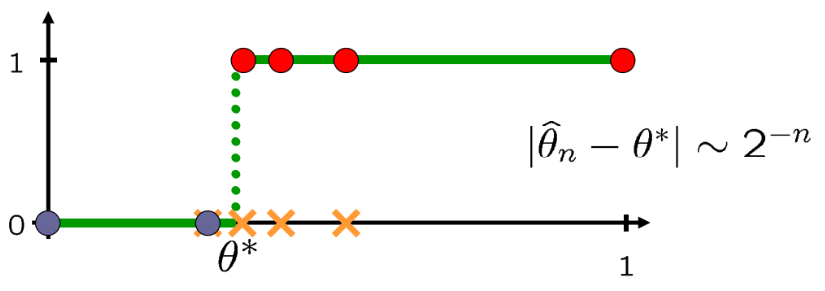
\includegraphics[width=4in]{img/bs.png}
\caption{Задача линейного разделения. Двоичный поиск}
\end{figure}

\emph{\textbf{Пример 2.}} Теперь рассмотрим пример, где сравниваются
результаты классификации с помощью логистической регрессии и ее
комбинации с активным обучением.

\begin{figure}[htbp]
\centering
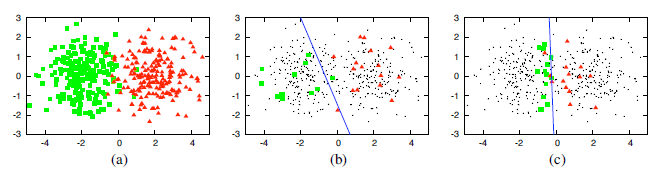
\includegraphics[width=6in]{img/example.png}
\caption{Пример работы обычной логистической регрессии (b) и
логистической регрессии с активным обучением (с)}
\end{figure}

На подграфике (a) изображены 400 точек, относящихся к одной из двух
меток, сгенерированных из двух различных двумерных гауссовских
распределений с одинаковой дисперисией (по 200 из каждого
распределения).

На подграфике (b) изображена разделящая прямая, построенная
логистической регрессией по 30 точкам, выбранных н.о.р. из пула всех
данных. Точность классификации 70\%. На следующем графике изображена
разделящая прямая, построенная логистической регрессией с активным
обучением по 30 точкам, выбранных по степени неуверенности. Точность
классификации 90\%.

Это пример еще раз подтверждает, что для активного обучения нужно
меньшее кол-во точек, чтобы обучится до приемлемой точности.

\subsection{Постановка задачи активного
обучения}

Пусть 
\(x_i\) --- объекты, \(y_i\) --- ответы (метки),  \(L_0 = \{(x_i, y_i)\}_i\) --- размеченные данные, \(U_0 = \{x_i\}_i\) --- неразмеченные данные. 

\textbf{Задача}: обучить модель по размеченным данным, минимизируя число вызовов оракула.

\textbf{Вход}: оракул, максимальное число вызовов
оракула \(K\), размеченные данные \(L_0\), неразмеченные данные \(U_0\).

\textbf{Алгоритм}: Обучить модель на \(L_0\). Для
\(k = 0, 1, \ldots, K - 1\):
\begin{enumerate}
\item
согласно стратегии, зависящей от модели, выбрать \(x_{k + 1} \in U_k\);
\item
узнать
для него \(y_{k + 1}\);
\item
получить оптимальное \(\theta_k\) на
тренировочных данных
\(L_{k + 1} := L_{k} \cup \{(x_{k + 1}, y_{k + 1})\}\).
\end{enumerate}

\emph{\textbf{Замечание 1}}:
Как упоминалось выше, основная идея
активного обучения --- выбирать наиболее информативные (с учетом
модели) объекты для разметки, чтобы кол-во вызовов оракула было
минимально. Стратегии выбора являются эвристиками,
потому что понятие ``наиболее информативные'' нельзя в общем случае
формализовать, результаты об оптимальности конкретной стратегии можно
получить разве что в каком-то отдельном частном случае.

\emph{\textbf{Замечание 2}}: Конечно, на каждой итерации можно (даже
нужно, потому что обучение модели может быть недешевой операцией)
запрашивать метки не для одного объекта \(x_{k + 1}\), а для нескольких
\(\{x_{k + 1}^{(i)}\}_{i = 1}^{m}\) и дообучать модель на
\(L_{k} \cup \{(x_{k + 1}^{(i)}, y_{k + 1}^{(i)})\}_{i = 1}^{m}\).

\emph{\textbf{Замечание 3}}: Как выбирать начальное множество \(L_0\)?
Наивный способ --- равномерно из неразмеченных данных, а можно
использовать специфику решаемой задачи. Например, для задач
классификации предварительно сделать кластеризацию и взять центры
кластеров.

\subsection{Стратегии выбора объектов для
разметки}

В активном обучении выделяют три типа источников неразмеченных данных:

\begin{itemize}
\item
  Семплирование из пула (pool-based sampling) --- есть некоторая
  коллекция неразмеченных данных, и из нее достаются объекты для запроса
  метки у оракула;
\item
  Семплирование из потока (stream-based selective sampling) --- есть
  поток данных, в каждый момент времени доступен один объект,
  принимается решение, отобрать этот объект для разметки или нет;
\item
  Генерация запросов (query sampling) --- обучающий алгоритм сам строит
  объекты для разметки.
\end{itemize}

Семплирование из пула наиболее встречающееся, и все перечисленные
стратегии относятся к этому типу семплирования.

Далее будем считать, что мы находимся в условиях задачи классификации,
но подобные варианты стратегий можно сформулировать и для задач
регрессии.

Введем обозначение \(\varphi_{\theta}(x)\) для функционала-эвристики,
оценивающего прирост качества модели при добавлении \(x\) к
тренировочным данным, так что
\(x^* = \arg\max_{x \in U} \varphi_{\theta}(x)\) --- следующая точка для
разметки;

\paragraph{Стратегия 1: выбор по степени неуверенности (uncertainty
sampling).}

Идея: давайте добавлять к тренировочным данным те объекты, в которых
модель больше всего неуверена.

Пусть \(P_{\theta}(y|x)\) --- апостериорная вероятность того, что \(x\)
относится к классу \(y\). В случае бинарной классификации с \(y = 0, 1\)
функционал-эвристику можно выбрать так
\(\varphi_{\theta}(x) = -|P_{\theta}(y = 0|x) - 0.5|\). Другими словами,
берем те \(x\), которые модель \(\theta\) относит к классу \(0\) с
вероятностью, наиболее близкой к \(0.5\) (то есть вероятность, что \(x\)
в классе \(1\) тоже близка к \(0.5\)).

В случае, когда классов больше, чем два:

\begin{enumerate}
\def\labelenumi{\alph{enumi})}
\item
  \(\varphi_{\theta}(x) = 1 - P_{\theta}(y^*|x)\), где \(y^* = y^*(x)\)
  --- наиболее вероятный класс для \(x\). Максимизация этой величины по
  \(x\) эквивалента \(\min_x\max_{y\in Y} P_{\theta}(y|x)\). Только
  здесь не учитываются вероятности \(P_{\theta}(y|x)\) на других метках,
  поэтому был предложен следующий подход.
\item
  \(\varphi_{\theta}(x) = P_{\theta}(y^*_2|x) - P_{\theta}(y^*_1|x)\),
  где \(y^*_i = y^*_i(x)\) --- \(i\)-й вероятный класс для \(x\). Здесь
  \emph{минимизируется} зазор между двумя лучшими предсказаниями \(y_1\)
  и \(y_2\). Но если меток очень много, лучше использовать следующий
  функционал:
\item
  \(\varphi_{\theta}(x) = - \sum_{y \in Y} P_{\theta}(y|x) \log P_{\theta}(y|x)\)
  --- не что иное, как энтропия. Вспомните, что ее максимум достигается
  на равномерном распределении.
\end{enumerate}

Ниже на тепловых картах сравниваются значения функционалов-эвристик
a)-с) (обратите внимание, что тепловые шкалы на трех графиках разные). Значения построены на двумерном симплексе с координатами вершин \((1, 0, 0),\, (0, 0, 1), (0, 1, 0)\), так как сумма вероятностей по всем классам равна \(1\).
Объекты, относительно которых модель больше всего неуверена, находятся в
центре, так как для них все апостериорные вероятности
\(P_{\theta}(y_i|x)\) примерно равны. Объекты, находящиеся ближе к
углам, считаются менее информативными, так как модель больше всего
уверена в предсказанным для них меткам.

\begin{figure}[htbp]
\centering
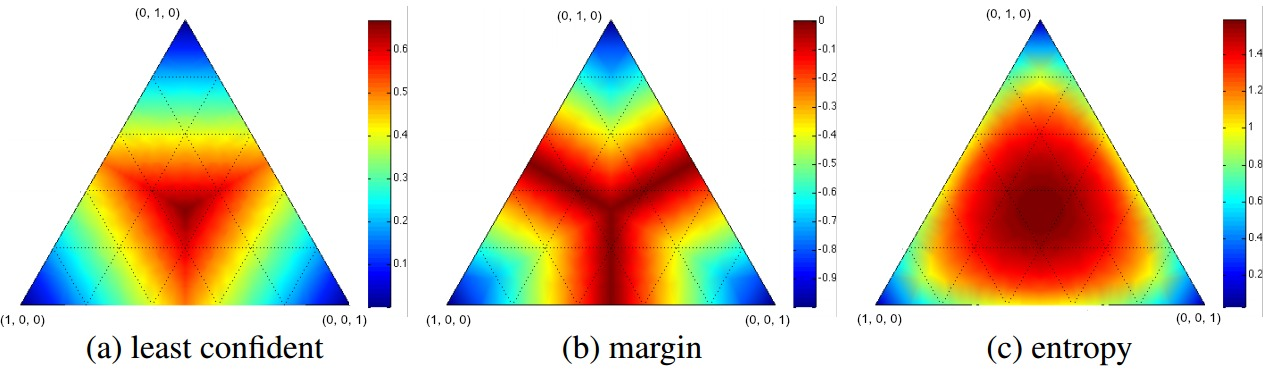
\includegraphics[width=6in]{img/hm.jpg}
\caption{Тепловые карты различных \(\varphi_k(x)\) в случае трех
классов. Синяя область --- наименее информативные объекты, красная
область --- наиболее информативные объекты согласно данной стратегии}
\end{figure}

Форму области красного цвета на каждом графике легко объяснить --- для
a) она имеет форму треугольника, так как значение функционала
определяется вероятностью \(P_{\theta}(y^*|x)\), для b) область
сосредоточена вдоль перпендикуляров от центра треугольника, так как она
соответствует равенству \(P_{\theta}(y^*_1|x)\) и
\(P_{\theta}(y^*_2|x)\). Что касается c), то в этом функционале
учитываются все априорные вероятности, и если для точки \(x\)
вероятность \(P_{\theta}(y|x)\) мала для некоторого \(y\) (такие \(x\)
располагаются вдоль сторон), то эта точка не включатся в число
информативных по стратегии c) (так как модель считает, что этот объект
не относится к тому классу).

\paragraph{Стратегия 2: отбор комитетом (query by
committee).}

\emph{Комитетом моделей} будем называть набор моделей, обученных на
одном и том же множестве \(L\). Обозначение ---
\(C_L = \{\theta_1,\ldots,\theta_m\}\). Идея стратегии: выбирать объекты
с наибольшей \emph{несогласованностью} комитетов моделей.

Пусть
\(V(y, x) = |{\theta \in C_{L}: y_{\theta}(x) = y}|\) --- количество
  моделей из комитета \(C_{L}\), выбравших \(y\),  \(\hat{P}(y|x) = V(y, x) / |C_{L}|\) --- соответственно доля моделей,
  выбравших \(y\).

Тогда несогласованность можно определить через
\(\varphi_{\theta}(x) = - \sum_{y \in Y} \hat{P}(y|x) \log \hat{P}(y|x)\)
--- энтропию голосующей вероятности.

Как уже говорилось, максимум энтропии достигается на равномерном
распределении, значит, максимизация этого функционала соответсвует
выбору объекта, для которого \(V(y, x)\) примерно равны для каждого
\(y\).

\paragraph{Стратегия 3: Сокращение пространства решений (version space
reduction).}

Идея этого подхода заключается в уменьшении пространствами решений
(version space). Под пространством решений в общем случае понимают
множество гипотез, которые согласуются с текущими тренировочными
данными. Понятие получается довольно размытое, но в задаче классификации
гипотезы \emph{связаны} с всевозможными разделяющими гиперплоскостями и
т.п.

\begin{figure}[htbp]
\centering
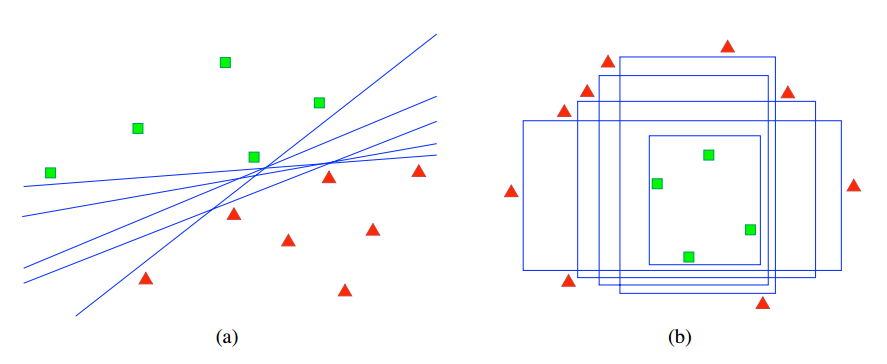
\includegraphics[width=6in]{img/vs.png}
\caption{Примеры пространств решений}
\end{figure}

Поскольку пространство решений это очень широкое понятие, то стратегии
его уменьшения можно описать только на примере конкретной задачи. Ниже
приведен пример, как комбинируется SVM и активное обучение, и уменьшение
пространства решений его ключевая идея.

\paragraph{Стратегия 4: ожидаемое влияние на модель (expected model
change).}

Идея: будем искать такой объект, добавление которого в обучающее
множество приведет к наибольшему \emph{изменению} параметра модели
\(\theta\). Само изменение будем мерять с помощью нормы градиента
функционала обучения \(\ell_{\theta}(L)\), где \(L\) --- обучающее
множество.

Нам нужно посчитать влияние на модель, но мы не знаем метку на \(x\) из
неразмеченного множества \(U\). Однако у нас есть апостриорное
распределение \(P_{\theta}(y|x)\), поэтому будем считать взвешенную
сумму
\(\varphi_{\theta}(x) = \sum_{y \in Y} P_{\theta}(y|x) \cdot \| \nabla\ell_{\theta}(L \cup \{(x, y)\})\|\),
другими словами, мат. ожидание нормы градиента.

Вспомните, что \(\nabla\ell_{\theta}(L) = 0\) (\(\theta\) оптимум на
обучающем множестве \(L\)), поэтому можно воспользоваться следующим
приближением
\(\nabla\ell_{\theta}(L \cup \{(x, y)\}) \approx \nabla\ell_{\theta}(\{(x, y)\})\)
для оптимизации вычислений.

\paragraph{Стратегия 5: ожидаемое уменьшение ошибки (expected error
reduction).}

Идея: максимизация уверенности на остальных объектах в неразмеченном
множестве.

Пусть \(\theta_+(x, y)\) --- оптимальный вектор параметров после
дообучения модели на \(L \cup \{(x, y)\}\), а \(y^* = y^*(z)\) ---
наиболее вероятный класс для \(z\) в модели, обученной на \(L\).

Рассмотрим функционал
\(\varphi_{\theta}(x) = - \sum_{y \in Y} P_{\theta}(y|x) \sum_{z \in U} (1 - P_{\theta_+(x, y)}(y^*|z))\),
его максимизация соответствует минимизации
\(\sum_{y \in Y} P_{\theta}(y|x) \sum_{z \in U} (1 - P_{\theta_+(x, y)}(y^*|z))\).
То есть находим \(x\), добавление которого увеличивает
\(P_{\theta_+(x, y)}(y^*|z))\) (делает как можно ближе к \(1\)) для всех
неразмеченных \(z\). Так как метку для \(x\) мы не знаем, то делаем
усреднение по всем \(y\).

\emph{\textbf{Замечание 4}}: В стратегиях выбор по степени неуверенности,
отбор комитетом, ожидаемое влияние на модель к числу информативных
объектов могут попасть аутлаеры. Поэтому их нужно исключить заранее, или
рассмотривать не \(\max_{x \in U} \varphi_{\theta}(x)\), а
\(\max_{x \in U} \varphi_{\theta}(x)\cdot \big(\frac{1}{|U|}\sum_{z \in U}\rho(x, z)\big)^{\beta}\),
где \(\rho\) --- это некоторая мера близости объектов, \(\beta\) ---
нормировочный коэффициент, чтобы контролировать величину весов.
Последняя стратегия устойчива к выбросам.

\subsection{Активное обучение в
SVM}

Посмотрим, как активное обучение комбинируется с классическими методами
классификации, таким как SVM. Описанный ниже метод относится к статье
\cite{TongKoller}, краткий обзор других статей на эту тему можно
найти в \cite{Settles}.

Будем предполать, что:

\begin{itemize}
\item
  данные линейно разделимы (но подход можно адаптировать под допущение
  ограниченного кол-ва ошибок, применять kernel trick, как это сделано в
  SVM);
\item
  класса два, их метки \(1\) и \(-1\).
\end{itemize}

\paragraph{Напоминание.}

В обычном SVM ищется классификатор вида
\(f(x) = {\rm sign}(\langle x, w \rangle - w_0)\) и решается
оптимизационная задача \(\|w\|^2/2 \to \min_{w, w_0}\) при условиях
\(y_i(\langle x_i, w \rangle - w_0) \geq 1\), где \(w, w_0\) ---
параметры алгоритма.

Величина \(|\langle x_i, w \rangle - w_0|/\|w\|\) --- это расстояние от
точки \(x_i\) до разделяющей гиперплоскости
\(\langle x, w \rangle - w_0 = 0\), поэтому когда минимизируется
\(\|w\|\), максимизируется зазор между \emph{опорными} гиперплоскостями,
которые проходят через ближайшие к разделяющей гиперплоскости \(x_i\).
Можно считать, что \(\|w\| = 1\), тогда оптимизационную задачу можно
переписать как
\(\min_i y_i (\langle x_i, w \rangle - w_0) \to \max_{w, w_0}\) при
условиях \(\|w\| = 1\) и \(y_i(\langle x_i, w \rangle - w_0) \geq 1\).

\paragraph{О пространстве
решений.}

По определению пространством решений будет являться
\(\mathcal{V} = \{f |\, y_if(x_i) > 0,\, i = 1 \ldots n\}\). Поскольку
между \(f\) и \(w\) существует биекция, то можно считать, что
\(\mathcal{V} = \{w\,|\, \|w\| = 1,\, y_i (\langle x_i, w \rangle - w_0) > 0,\, i = 1\ldots n \}\).

Обозначим за \(Area(\mathcal{V})\) площадь пространства решений.

\paragraph{Теоретическое отступление, результат которого используется
дальше.}

Если предположить, что \(\|x_i\| = 1\), то
\(\min_i y_i(\langle x_i, w \rangle - w_0) = \min_i |\langle w, y_i x_i\rangle - y_i w_0| = \min_i |\langle w, y_i x_i\rangle - y_i w_0|/\|y_ix_i\|\),
а значит зазор между гиперплоскостями также равен минимальному
расстоянию от \(w\) до гиперплоскости
\(\langle v, y_i x_i\rangle - y_i w_0 = 0\) относительно \(v\).

Отсюда следует, что оптимальный параметр \(w\) --- это центр гиперсферы
наибольшего радиуса в \(\mathcal{V}\), которая бы не пересекалась ни с
одной из гиперплоскостей полном пространстве.

\begin{figure}[htbp]
\centering
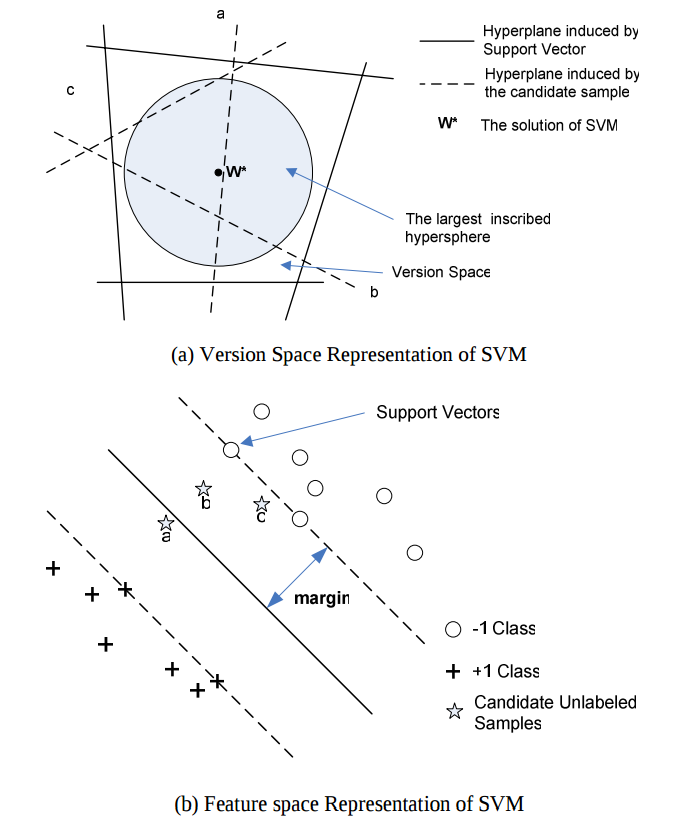
\includegraphics[width=5in]{img/svm+al.png}
\caption{Активное обучение в SVM}
\end{figure}

\paragraph{Об активном
обучении.}

Обозначим за \(\mathcal{V}_k(\ell)\) пространство решений после \(k\) итераций активного обучения,
который использует стратегию \(\ell\).

\textbf{Лемма, см. \cite{TongKoller}}:
Рассмотрим последовательность \(\{Area(\mathcal{V}_k(\ell))\}_{k \geq 1}\).
Пусть  \(\ell^*\) это стратегия деления \(Area(\mathcal{V}_k)\)
пополам, тогда для любой другой стратегии
\(\ell\) выполняется неравенство:
\[\sup_{P \in \mathcal{P}} {\rm E}_P[Area(\mathcal{V}_k(\ell^*))] \leq \sup_{P \in \mathcal{P}} {\rm E}_P[Area(\mathcal{V}_k(\ell))]\]

для любого \(k \geq 1\), где \(\mathcal{P}\) --- множество всех условных
распределений \(P(y|x)\). При этом строгое неравенство достигается, если
существует итерация \(j \in 1,\ldots, k\), такая, что \(\ell\) не делит
пространство решений \(\mathcal{V}_{j - 1}\) пополам.


Пусть \(w_k\) --- центр гиперсферы наибольшего радиуса, которая вписана
в пространство решений \(\mathcal{V}_k\). Предлагается три способа
делить пространство решений так, чтобы площади полученных областей были
примерно равны:

\begin{itemize}
\item
  \emph{Simple Margin}. Теперь перебирая все неразмеченные объекты
  \(x\), выберем тот, для которого соответсвующая гиперплоскость ближе
  всего к центру \(w_k\). По отступлению выше такой \(x_k\) находится
  ближе всего к разделяющей гиперплоскости в пространстве объектов.
\end{itemize}

\begin{figure}[htbp]
\centering
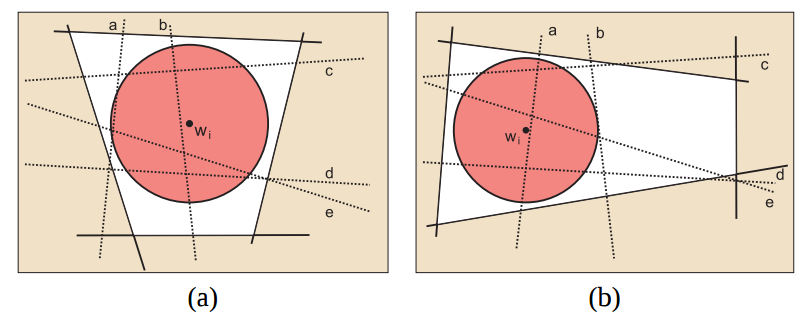
\includegraphics[width=5in]{img/simplemargin.png}
\caption{Simple Margin. (a) выбирается ближайшая гиперплоскость
b. (b) выбирается ближайшая гиперплоскость a}
\end{figure}

Обозначим за \(m_k\) радиус гиперсферы. Рассмотрим неразмеченный объект
\(x\), 
\(\mathcal{V}_k^- = \mathcal{V}_k \cap \{w\,|\, \langle w, x\rangle < 0\}\)
и
\(\mathcal{V}_k^+ = \mathcal{V}_k \cap \{w\,|\, \langle w, x\rangle > 0\}\) --- подпространства в
пространсве решений, соответствующие отрицательной и положительной метке
\(x\). Теперь обозначим за \(m^-_k\) и \(m^+_k\) радиусы вписанных в
\(\mathcal{V}_k^-\) и \(\mathcal{V}_k^+\) сфер.


\begin{itemize}
\item
  \emph{MaxMin Margin}. Эта стратегия предлагает искать
  \(\arg\max_x \min\{m^+_k, m^-_k\}\). Так как \(m_k\) cвязан с
  \(Area(\mathcal{V}_k)\), то на самом деле максимизируется
  \(\min\{Area(\mathcal{V}_k^+), Area(\mathcal{V}^-_k)\}\), тогда
  \(Area(\mathcal{V}_k^+)\) и \(Area(\mathcal{V}^-_k)\) будут
  максимально близки.
\item
  \emph{Ratio Margin}. В этой стратегии ищется
  \(\arg\max_x \min\{m^+/m^-, m^-/m^+\}\), она объясняется так же, как и
  стратегия MaxMin Margin.
\end{itemize}

\begin{figure}[htbp]
\centering
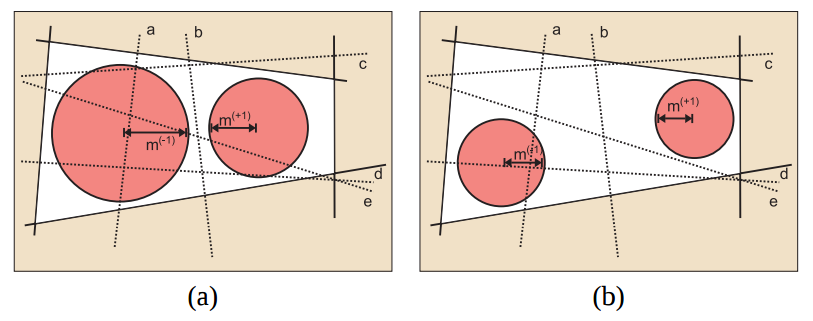
\includegraphics[width=5in]{img/maxminmargin.png}
\caption{(a) MaxMin Margin --- выбирается гиперплоскость b. (b)
Ratio Margin --- выбирается гиперплоскость e}
\end{figure}

\subsection{Недостатки активного
обучения}

Стратегии активного обучения устроены так, что они рекомендуют точки,
лежащие, например, вблизи разделяющей гиперплоскости в текущей модели.
Это хорошо работает, если нет крупных областей, где модель бы ошибалась.
Таким образом, у алгоритма среди данных есть необследованные участки,
что повышается ошибку на тестовых данных.

Возникает так называемая exploration-exploitation dilemma, но есть
приемы, связанные с применением контекстных бандитов (см. \cite{Bouneffouf1}) и случайным изучением всего неразмеченного множества (см.
\cite{Bouneffouf2}), которые не увеличивают время обучения так, что сама
идея активного обучения теряет смысл.

\bibliography{bibliography}
\bibliographystyle{gost2008}

\end{document}
